%%%%%%%%%%%%%%%%%%%%%%%%%%%%%%%%%%%%%%%%%
% Version 2.0 (10/10/16)
%
% Original author:
% Frits Wenneker (http://www.howtotex.com)
% Modifier:
% Altug Yildirim
%
% License:
% CC BY-NC-SA 3.0 (http://creativecommons.org/licenses/by-nc-sa/3.0/)
%
%%%%%%%%%%%%%%%%%%%%%%%%%%%%%%%%%%%%%%%%%

%----------------------------------------------------------------------------------------
%	PACKAGES AND OTHER DOCUMENT CONFIGURATIONS
%----------------------------------------------------------------------------------------

\documentclass[paper=a4, fontsize=11pt]{scrartcl} % A4 paper and 11pt font size

\usepackage[T1]{fontenc} % Use 8-bit encoding that has 256 glyphs
\usepackage{fourier} % Use the Adobe Utopia font for the document - comment this line to return to the LaTeX default
\usepackage[english]{babel} % English language/hyphenation
\usepackage{amsmath,amsfonts,amsthm} % Math packages
\usepackage{adjustbox} %for adjusting the table size
\usepackage[affil-it]{authblk}  %for adjusting the author and affilition font size
\usepackage[font=scriptsize]{caption} %for adjusting the font size of captions
\usepackage{multirow} %for merging the header cells
\usepackage{hhline} %for merging the header cells
\usepackage{listings} %for code display
\usepackage{color} %for code display
\lstset{frame=tb,
  language=Python,
  aboveskip=3mm,
  belowskip=3mm,
  showstringspaces=false,
  columns=flexible,
  basicstyle={\small\ttfamily},
  numbers=none,
  numberstyle=\tiny\color{gray},
  keywordstyle=\color{blue},
  commentstyle=\color{green},
  stringstyle=\color{red},
  breaklines=true,
  breakatwhitespace=true,
  tabsize=1
} %for code didplay

\usepackage{graphicx} %for inserting graphics
\graphicspath{ {images/} } %for determining the folder where the graphic is

\usepackage{sectsty} % Allows customizing section commands
\allsectionsfont{\centering \normalfont\scshape} % Make all sections centered, the default font and small caps
\newif\ifcomment
 \commenttrue % Show comments

\renewcommand\Authfont{\fontsize{12}{14.4}\selectfont}
\renewcommand\Affilfont{\fontsize{9}{10.8}\itshape}

\usepackage{fancyhdr} % Custom headers and footers
\pagestyle{fancyplain} % Makes all pages in the document conform to the custom headers and footers
\fancyhead{} % No page header - if you want one, create it in the same way as the footers below
\fancyfoot[L]{} % Empty left footer
\fancyfoot[C]{} % Empty center footer
\fancyfoot[R]{\thepage} % Page numbering for right footer
\renewcommand{\headrulewidth}{0pt} % Remove header underlines
\renewcommand{\footrulewidth}{0pt} % Remove footer underlines
\setlength{\headheight}{13.6pt} % Customize the height of the header

\numberwithin{equation}{section} % Number equations within sections (i.e. 1.1, 1.2, 2.1, 2.2 instead of 1, 2, 3, 4)
\numberwithin{figure}{section} % Number figures within sections (i.e. 1.1, 1.2, 2.1, 2.2 instead of 1, 2, 3, 4)
\numberwithin{table}{section} % Number tables within sections (i.e. 1.1, 1.2, 2.1, 2.2 instead of 1, 2, 3, 4)

\setlength\parindent{0pt} % Removes all indentation from paragraphs - comment this line for an assignment with lots of text

%----------------------------------------------------------------------------------------
%	TITLE SECTION
%----------------------------------------------------------------------------------------

\newcommand{\horrule}[1]{\rule{\linewidth}{#1}} % Create horizontal rule command with 1 argument of height

\title{	
\normalfont \normalsize 
\textsc{Istanbul Technical University, Mathematics Department \\ Numerical Methods for Partial Differential Equations I} \\ [25pt]
\horrule{0.5pt} \\[0.4cm] % Thin top horizontal rule
\large Homework I \\ % The assignment title
\horrule{0.5pt} \\[0.4cm] % Thick bottom horizontal rule
}

\author{Haydar Altu\u{g} Y{\i}ld{\i}r{\i}m \\ 509161108} 

\date{\normalsize\today} % Today's date or a custom date

\begin{document}

\maketitle % Print the title

\section{Numerical and Analytical Derivation of Functions and Relative Errors}

Find the numerical(forward, backward and central) and analytical solutions of the functions $u_1=sin(x)$ and $u_2 = e ^{ {x^ 2}} $ at the point $x=1$ and calculate the percentage error.

%the table below is made with the help of the site; http://ericwood.org/excel2latex/ with addition of captions and adjustbox
\begin{table}[ht]
\centering
\begin{adjustbox}{width=1\textwidth}
\small
\begin{tabular}{ | l | l | l | l | l | l | l | l | l | l | l | l | l | }
\hline
	$u_1$ & \multicolumn{4}{c|}{forward differences}  & \multicolumn{4}{c|}{backward differences} &  \multicolumn{4}{c|}{central differences}   \\ \hline
	$\Delta$ x & analytic & numeric & error(\%) & p($\varepsilon$) & analytic & numeric & error(\%) & p($\varepsilon$) & analytic & numeric & error(\%) & p($\varepsilon$) \\ \hline
	0.1 & 0.5403 & 0.4973 & 7.9585 & -0.9008 & 0.5403 & 0.5814 & 7.6068 & -0.8812 & 0.5403 & 0.5393 & 0.1665 & 0.7783 \\ \hline
	0.05 & 0.5403 & 0.519 & 3.9422 & -0.4579 & 0.5403 & 0.5611 & 3.8497 & -0.4499 & 0.5403 & 0.54 & 5.5524E-2 & 0.9650 \\ \hline
	0.01 & 0.5403 & 0.536 & 0.7958 & 4.9583E-2 & 0.5403 & 0.5444 & 0.7773 & 5.4692E-2 & 0.5403 & 0.5402 & 1.8508E-2 & 0.8663 \\ \hline
	5E-3 & 0.5403 & 0.5381 & 0.4071 & 0.1695 & 0.5403 & 0.5423 & 0.3886 & 0.1783 & 0.5403 & 0.5403 & 0 &  \\ \hline
	1E-3 & 0.5403 & 0.5397 & 9.2541E-2 & 0.3445 & 0.5403 & 0.5406 & 7.4032E-2 & 0.3768 & 0.5403 & 0.5403 & 0 &  \\ \hline
\end{tabular}
\end{adjustbox}
\caption{$u_1 = sin(x)$ calculations}
\end{table} 

\begin{table}[ht]
\centering
\begin{adjustbox}{width=1\textwidth}
\small
\begin{tabular}{ | l | l | l | l | l | l | l | l | l | l | l | l | l |}
\hline
	$u_2$ & \multicolumn{4}{c|}{forward differences}  & \multicolumn{4}{c|}{backward differences} &  \multicolumn{4}{c|}{central differences}   \\ \hline
	$\Delta$ x & analytic & numeric & error(\%) & p($\varepsilon$) & analytic & numeric & error(\%) & p($\varepsilon$) & analytic & numeric & error(\%) & p($\varepsilon$) \\ \hline
	0.1 & 5.4364 & 6.352 & 16.8398 & -1.2263 & 5.4364 & 4.7037 & 13.4792 & -1.1296 & 5.4364 & 5.5278 & 1.6793 & -0.2251 \\ \hline
	0.05 & 5.4364 & 5.868 & 7.937 & -0.6914 & 5.4364 & 5.0503 & 7.1019 & -0.6543 & 5.4364 & 5.4592 & 0.4175 & 0.2915 \\ \hline
	0.01 & 5.4364 & 5.5191 & 1.5175 & -9.0567E-2 & 5.4364 & 5.3559 & 1.4825 & -8.5507E-2 & 5.4364 & 5.4374 & 1.6554E-2 & 0.8905 \\ \hline
	5E-3 & 5.4364 & 5.4775 & 0.7541 & 5.3252E-2 & 5.4364 & 5.395 & 0.7449 & 5.5568E-2 & 5.4364 & 5.4367 & 3.6788E-3 & 1.0579 \\ \hline
	1E-3 & 5.4364 & 5.4447 & 0.1508 & 0.2738 & 5.4364 & 5.4283 & 0.1489 & 0.2756 & 5.4364 & 5.4364 & 0 &  \\ \hline
\end{tabular}
\end{adjustbox}
\caption{$u_2 = e ^{ {x^ 2}} $ calculations} 
\end{table} 

p($\varepsilon$) calculated from the following arguments;

\begin{align}
Error \approx \Delta x \\
E=C(\Delta x)^p \\
log(E) \approx log(C(\Delta x)^p) \\
\approx log(C)+log((\Delta x)^p) \\
log(E) \approx log(C)+p*log(\Delta x) \\
p = log(E)/log(\Delta x)
\end{align}

If we plot the $ log(E)$ and $log(\Delta x) $ and calculate the slopes ;

\begin{figure}[h]
\centering
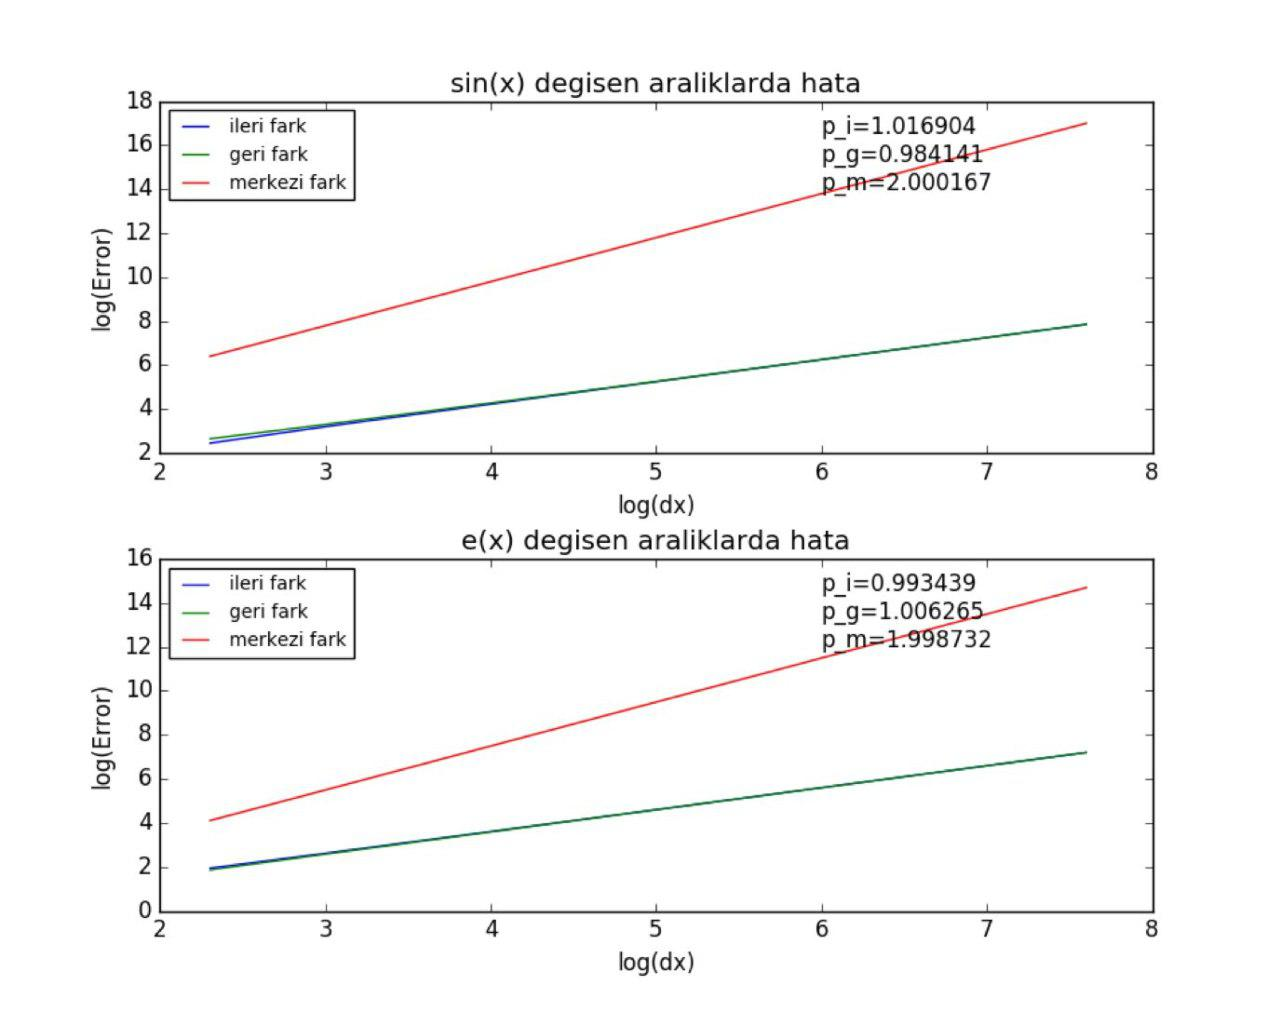
\includegraphics[scale=0.5]{graph1}
\end{figure}

\ifcomment
Code that written for the values in the table and to plot the graph;

\begin{lstlisting}
#!/usr/bin/python

from math import sin, exp
from numpy import *
import matplotlib.pyplot as plt

#Fonsksiyonlar

def fsin(x):
	return sin(x)

def fexp(x):
	return exp(x**2)

#Initialization

exact_sin = cos(1)
exact_e = 2*1*exp(1**2)

d = [1e-1,5e-2,1e-2,5e-3,1e-3,5e-4]

r_sin=ones((3,size(d)))
r_e=ones((3,size(d))) 

error_sin=ones((3,size(d)))
error_e=ones((3,size(d)))

perror_sin=ones((3,size(d)))
perror_e=ones((3,size(d)))


##Sayisal turevler 

def ileri (f, x, dx):
	return (f(x+dx)-f(x))/dx

def geri (f,x,dx):
	return (f(x) - f(x-dx))/dx

def central (f,x,dx):
	return (f(x+dx)-f(x-dx))/(2*dx)

#####
def op(f, d, r, error,perc_error, exact, x):	
	
	for i in range(size(d)):
		r[0][i]=ileri(f,x,d[i])
		r[1][i]=geri(f,x,d[i])
		r[2][i]=central(f,x,d[i])

		error = abs((exact-r)/r)
		perc_error = error*100
	return r , error, perc_error

###Uygulama

r_sin, error_sin, perror_sin = op(fsin, d, r_sin, error_sin, perror_sin, exact_sin, 1)
r_e, error_e, perror_e = op(fexp, d, r_e, error_e, perror_e, exact_e, 1)

#p ler



##Plot
x = abs(log(d))
#Sin turevi icin eksenler
y_s = abs(log(error_sin[0]))
y1_s = abs(log(error_sin[1]))
y2_s = abs(log(error_sin[2]))

p_s, z = polyfit(x, y_s, 1)
p1_s, z = polyfit(x, y1_s, 1)
p2_s, z = polyfit(x, y2_s, 1)

plt.figure(1)
plt.subplot(211)
plt.xlabel('log(dx)')
plt.ylabel('log(Error)')
plt.title('sin(x) degisen araliklarda hata')

plt.plot(x,y_s,x,y1_s,x,y2_s)

plt.text(6, 14, 'p_i=%f\np_g=%f\np_m=%f'%(p_s,p1_s,p2_s))

plt.legend(['ileri fark','geri fark','merkezi fark'],loc='best',fontsize=10)

#E fonk

y_e = abs(log(error_e[0]))
y1_e = abs(log(error_e[1]))
y2_e = abs(log(error_e[2]))

p_e, z = polyfit(x, y_e, 1)
p1_e, z = polyfit(x, y1_e, 1)
p2_e, z = polyfit(x, y2_e, 1)

plt.figure(1)
plt.subplot(212)
plt.xlabel('log(dx)')
plt.ylabel('log(Error)')
plt.title('e(x) degisen araliklarda hata')

plt.plot(x,y_e,x,y1_e,x,y2_e)

plt.text(6, 12, 'p_i=%f\np_g=%f\np_m=%f'%(p_e,p1_e,p2_e))

plt.legend(['ileri fark','geri fark','merkezi fark'],loc='best',fontsize=10)
plt.show()
\end{lstlisting}
\fi

\end{document}